\documentclass[12pt]{article}
\usepackage{fullpage}
\usepackage[utf8]{inputenc}
\usepackage{pict2e}
\usepackage{amsmath}
\usepackage{enumitem}
\usepackage{eurosym}
\usepackage{pict2e}
\usepackage{mathtools}
\usepackage{amssymb, amsfonts, latexsym, cancel}
\setlength{\parskip}{0.3cm}
\usepackage{graphicx}
\usepackage{fontenc}
\usepackage{slashbox}
\usepackage{setspace}
\usepackage{gensymb}
\usepackage{accents}
\usepackage{adjustbox}
\setstretch{1.5}
\usepackage{bold-extra}
\usepackage[document]{ragged2e}
\usepackage{subcaption}
\usepackage{tcolorbox}
\usepackage{xcolor, colortbl}
\usepackage{wrapfig}
\usepackage{empheq}
\usepackage{array}
\usepackage{parskip}
\usepackage{arydshln}
\graphicspath{ {images/} }
\renewcommand*\contentsname{\color{black}Índice} 
\usepackage{array, multirow, multicol}
\definecolor{lightblue}{HTML}{007AFF}
\usepackage{color}
\usepackage{etoolbox}
\usepackage{listings}
\usepackage{mdframed}
\setlength{\parindent}{0pt}
\usepackage{underscore}
\usepackage{hyperref}
\usepackage{tikz}
\usepackage{tikz-cd}
\usetikzlibrary{shapes, positioning, patterns}
\usepackage{tikz-qtree}
\usepackage{biblatex}
\usepackage{pdfpages}
\usepackage{pgfplots}
\usepackage{pgfkeys}
\addbibresource{biblatex-examples.bib}
\usepackage[a4paper, left=1.5cm, right=1.5cm, top=1cm,
bottom=1.5cm]{geometry}
\everymath{\displaystyle}
\usetikzlibrary{decorations.pathreplacing}
\usepackage{titlesec}
\usepackage{titletoc}
\usepackage{tikz-3dplot}
\usetikzlibrary{decorations.pathreplacing}
\newcommand{\Ej}{\textcolor{lightblue}{\underline{Ejemplo}}}
\setlength{\fboxrule}{1.5pt}
\renewcommand{\arraystretch}{1.35}
\setlength{\arraycolsep}{0.3cm}

% Configura el formato de las secciones utilizando titlesec
\titleformat{\section}
{\color{red}\normalfont\LARGE\bfseries}
{Tema \thesection:}
{10 pt}
{}

% Ajusta el formato de las entradas de la tabla de contenidos
\addtocontents{toc}{\protect\setcounter{tocdepth}{4}}
\addtocontents{toc}{\color{black}}

\titleformat{\subsection}
{\normalfont\Large\bfseries\color{red}}{\thesubsection)}{1em}{\color{lightblue}}

\titleformat{\subsubsection}
{\normalfont\large\bfseries\color{red}}{\thesubsubsection)}{1em}{\color{lightblue}}

\newcommand{\bboxed}[1]{\fcolorbox{lightblue}{lightblue!10}{$#1$}}

\DeclareMathOperator{\N}{\mathbb{N}}
\DeclareMathOperator{\Z}{\mathbb{Z}}
\DeclareMathOperator{\R}{\mathbb{R}}
\DeclareMathOperator{\Q}{\mathbb{Q}}
\DeclareMathOperator{\K}{\mathbb{K}}
\DeclareMathOperator{\im}{\imath}
\DeclareMathOperator{\jm}{\jmath}
\DeclareMathOperator{\col}{\mathrm{Col}}
\DeclareMathOperator{\fil}{\mathrm{Fil}}
\DeclareMathOperator{\rg}{\mathrm{rg}}
\DeclareMathOperator{\nuc}{\mathrm{nuc}}
\DeclareMathOperator{\dimf}{\mathrm{dimFil}}
\DeclareMathOperator{\dimc}{\mathrm{dimCol}}
\DeclareMathOperator{\dimn}{\mathrm{dimnuc}}
\DeclareMathOperator{\dimr}{\mathrm{dimrg}}

\newcommand{\bu}[1]{\textcolor{lightblue}{\underline{#1}}}
\newcommand{\lb}[1]{\textcolor{lightblue}{#1}}
\newcommand{\db}[1]{\textcolor{blue}{#1}}
\newcommand{\rc}[1]{\textcolor{red}{#1}}
\newcommand{\tr}{^\intercal}

\renewcommand{\CancelColor}{\color{lightblue}}

\newcommand{\dx}{\:\mathrm{d}x}
\newcommand{\dt}{\:\mathrm{d}t}
\newcommand{\dy}{\:\mathrm{d}y}
\newcommand{\dz}{\:\mathrm{d}z}
\newcommand{\dth}{\:\mathrm{d}\theta}
\newcommand{\dr}{\:\mathrm{d}\rho}
\newcommand{\du}{\:\mathrm{d}u}
\newcommand{\dv}{\:\mathrm{d}v}
\newcommand{\tozero}[1]{\cancelto{0}{#1}}
\newcommand{\lbb}[2]{\textcolor{lightblue}{\underbracket[1pt]{\textcolor{black}{#1}}_{#2}}}
\newcommand{\dbb}[2]{\textcolor{blue}{\underbracket[1pt]{\textcolor{black}{#1}}_{#2}}}
\everymath{\displaystyle}

\begin{document}
\begin{enumerate}[label=\color{red}\textbf{\arabic*)}, leftmargin=*]
	\item \lb{Determinar el dominio de definición de las siguientes funciones:}
	
	$\db{f(x)=x-\sqrt{\dfrac{x+2}{x-1}}}$
	
	Para empezar, como hay un cociente debemos evitar que el denominador sea cero \begin{center}
		$x-1=0\longrightarrow\bboxed{x=1}$ No está en el dominio
	\end{center}
	Por otro lado, tenemos una raíz cuadrado y esto implica que la de dentro, debe ser positivo o cero: $\dfrac{x+2}{x-1}\ge0$
	\begin{center}
		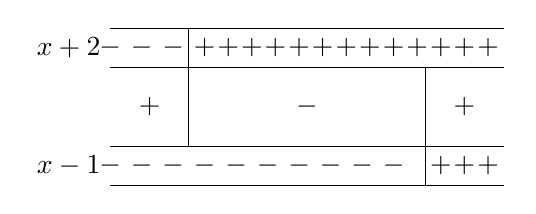
\begin{tikzpicture}
			\draw (-3,0) -- (2,0)
			(-3,-0.5) -- (2,-0.5)
			(-3,-1.5) -- (2,-1.5)
			(-3,-2) -- (2,-2);
			\node[left] at (-3,-0.25) {$x+2$};
			\node[left] at (-3,-1.75) {$x-1$};
			\foreach \x in {-3, -2.6, ..., -2.1}{
			\node at (\x, -0.25) {$-$};
			}
			\foreach \x in {-3, -2.6, ..., 0.8}{
			\node at (\x, -1.75) {$-$};
			}
			\foreach \x in {-1.8, -1.5, ..., 2}{
			\node at (\x, -0.25) {$+$};
			}
			\foreach \x in {1.2, 1.5, ..., 2}{
			\node at (\x, -1.75) {$+$};
			}
			\draw (-2,0) -- (-2,-1.5);
			\draw (1,-0.5) -- (1,-2);
			\node[circle] at (-2.5,-1) {+};
			\node[circle] at (1.5,-1) {+};
			\node[circle] at (-0.5,-1) {$-$};
		\end{tikzpicture}
	\end{center}
	$\dfrac{x+2}{x-1}\ge0\longrightarrow x\in(-\infty,-2]\cup(1,+\infty)$
	
	Por lo tanto el dominio de la función es: \[ \bboxed{\dom(f)=(-\infty,-2]\cup(1,+\infty)} \]
	\item \lb{Determinar el dominio de definición de las siguientes funciones:}
	
	$\db{f(x)=\sqrt[4]{\dfrac{x}{\log(x)}}}$
	
	Como hay un cociente entonces el denominador no puede ser cero: \begin{center}
		$\log(x)=0\longrightarrow\bboxed{x=1}$ No está en el dominio
	\end{center}
	Como hay un logaritmo, lo de dentro solo puede ser positivo: \[ \bboxed{x>0} \]Como tenemos una raíz cuarta (de grado par) entonces lo de dentro no puede ser negativo:
	
	\begin{minipage}{0.4\textwidth}
		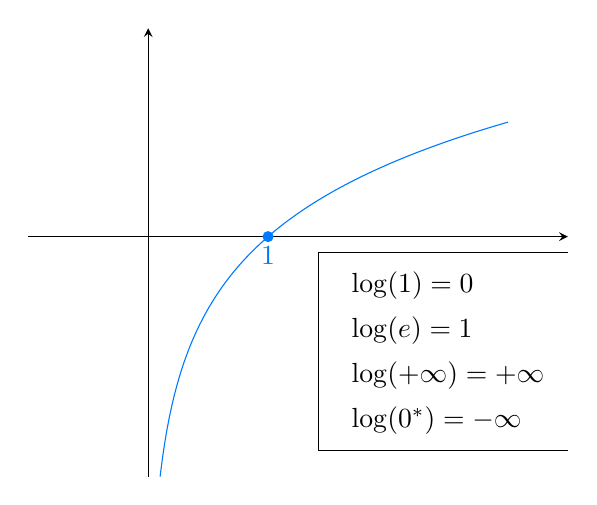
\begin{tikzpicture}
			\begin{axis}[xmin=-1, xmax=3.5, ymax=2, axis lines=center, xtick=\empty, ytick=\empty]
				\addplot[lightblue, domain=0.1:3, samples=150] {ln(x)};
				\fill[lightblue] (axis cs:1,0) circle (2pt) node[below] {$1$};
				\node[rectangle, draw=black] at (axis cs:2.5,-1.1) {$\begin{array}{l}
						\log(1)=0\\
						\log(e)=1\\
						\log(+\infty)=+\infty\\
						\log(0^*)=-\infty\\
					\end{array}$};
			\end{axis}
		\end{tikzpicture}
	\end{minipage}\qquad\begin{minipage}{0.45\textwidth}
	$\dfrac{x}{\log(x)}\ge0\longrightarrow x\in(1,+\infty)$
	\begin{center}
		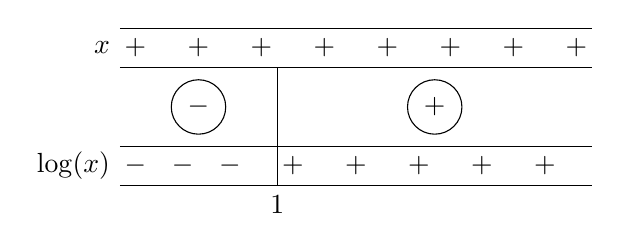
\begin{tikzpicture}[xscale=2]
			\draw (0,0) -- (3,0)
			(0,-0.5) -- (3,-0.5)
			(0,-1.5) -- (3,-1.5)
			(0,-2) -- (3,-2)
			;
			\foreach \x in {0.1, 0.5, ..., 3}{\node at (\x, -0.25) {$+$};}
			\foreach \x in {0.1, 0.4, ..., 0.8}{\node at (\x, -1.75) {$-$};}
			\foreach \x in {1.1, 1.5, ..., 3}{\node at (\x, -1.75) {$+$};}
			\draw (1,-0.5) -- (1,-2) node[below] {$1$};
			\node[circle, draw=black] at (0.5, -1) {$-$};
			\node[circle, draw=black] at (2, -1) {$+$};
			\node[left] at (0,-0.25) {$x$};
			\node[left] at (0,-1.75) {$\log(x)$};
		\end{tikzpicture}
	\end{center}
	Por lo tanto: \[ \bboxed{\dom(f)=(1,+\infty)} \]
	\end{minipage}
	\item \lb{Vamos a comprobar si la aplicación \[ \begin{aligned}
			f:&\R\longrightarrow\R\\
			&x\longmapsto f(x)=2x+1
		\end{aligned} \]es biyectiva, es decir, si es inyectiva y sobreyectiva.}
	
	\begin{minipage}{0.5\textwidth}
		Veamos si la aplicación $f(x)$ es inyectiva:
		\begin{itemize}[leftmargin=*]
			\item Sea: \[ f(x_1)=f(x_2)\longrightarrow2x_1+1=2x_2+1\longrightarrow\bboxed{x_1=x_2} \]Por lo tanto: $f(x)$ es inyectiva.
			\item Por otro lado: $\forall y\in\R\longrightarrow y=f(x)=2x+1$ 
			\begin{center}
				$2x=1-y\longrightarrow x=\dfrac{1-y}{2}$ Por lo tanto $\forall y\in\R$ existe un $x\in\R$ tal que $f(x)=y$$\longrightarrow f(x)$ es sobreyectiva.
			\end{center}
		\end{itemize}
		
	\end{minipage}\qquad\begin{minipage}{0.4\textwidth}
	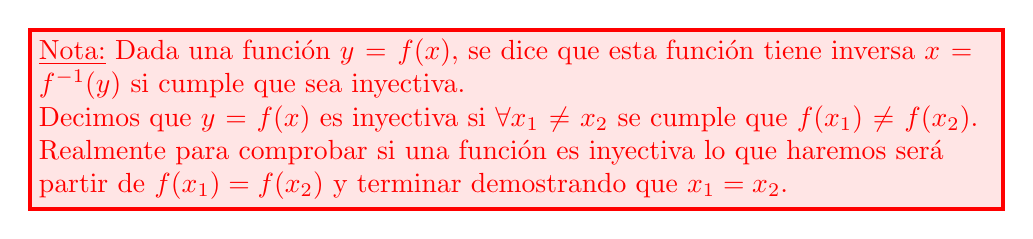
\begin{tikzpicture}
		\node[red, draw=red, fill=red!10, line width=1.5, text width=\linewidth] {\underline{Nota:} Dada una función $y=f(x)$, se dice que esta función tiene inversa $x=f^{-1}(y)$ si cumple que sea inyectiva.\\
		Decimos que $y=f(x)$ es inyectiva si $\forall x_1\neq x_2$ se cumple que $f(x_1)\neq f(x_2)$. Realmente para comprobar si una función es inyectiva lo que haremos será partir de $f(x_1)=f(x_2)$ y terminar demostrando que $x_1=x_2$.};
	\end{tikzpicture}
	\end{minipage}
	
	Entonces, como $f(x)$ es inyectiva y sobreyectiva en todo $\R$ podemos asegurar que $f(x)$ es biyectiva y por lo tanto existe su función inversa. \[ \begin{aligned}
		f^{-1}:&\R\longrightarrow\R\\
		&y\longrightarrow x=f^{-1}(y)=\dfrac{1-y}{2}
	\end{aligned} \]
	
\item \lb{Comprobar si la función $f:\R\longrightarrow\R$ con $f(x)=x^2$ tiene inversa.}

Para que tenga inversa debe ser inyectiva, y esto implica que para elementos diferentes debe tener diferentes y como: 
\begin{center}
	$\begin{rcases}
		f(1)=1\\
		f(-1)=1
	\end{rcases}$ No es inyectiva $\longrightarrow f(x)$ No tiene inversa
\end{center}
\item \lb{Dadas las siguientes funciones, averiguar en qué puntos son discontinuas y por qué.}

$\db{f(x)=\dfrac{x^2}{x-2}\text{ si }x\neq0,\, f(2)=0.}$

$f(x)=\begin{cases}
	\dfrac{x^2}{x-2} & \text{si }x\neq2\\
	0 & \text{si }x=2
\end{cases}$\\
$\forall x\neq2\:f(x)$ es continua por ser un cociente de funciones continuas con denominador distinto de cero.

Veamos ahora si es continua en $x=2$.

\begin{center}
	$\begin{rcases}
	\lim_{x\to2^-}\dfrac{x^2}{x-2}=\dfrac{4}{0^-}=-\infty\\
	\lim_{x\to2^+}\dfrac{x^2}{x-2}=\dfrac{4}{0^+}=+\infty\\
\end{rcases}$\quad\begin{minipage}{0.5\textwidth}
$f(x)$ No es continua en $x=2$, en concreto presenta en $x=2$ una discontinuidad inevitable de salto infinito. Diremos que $f(x)$ presenta en $x=2$ una asíntota vertical.
\end{minipage}\\
\begin{tikzpicture}
	\begin{axis}[xmin=-1, xtick=\empty, ytick=\empty, axis lines=center, xmax=4]
		\addplot[lightblue, line width=1.5, domain=2.1:2.2] {x^2/(x-2)};
		\addplot[lightblue, line width=1.5, domain=1.7:1.9] {x^2/(x-2)};
		\draw[lightblue] (axis cs:2,50) -- (axis cs:2,-50);
		\fill[lightblue] (axis cs:2,0) circle (2pt) node[ below right] {$2$};
	\end{axis}
\end{tikzpicture}
\end{center}
\item \lb{Determinar el dominio de definición de las siguientes funciones:}

$\db{f(x)=\dfrac{1}{\sqrt{1-e^x}}}$

Como es un cociente, debemos evitar que el denominador sea cero: \begin{center}
	$1-e^x=0\longrightarrow e^x=1\longrightarrow x=\ln(1)=0\longrightarrow\bboxed{x=0}$ No pertence el dominio
\end{center}
Como hay una raiz cuadrada, lo de dentro no puede ser negativo: \[ 1-e^x>0\longrightarrow e^x<1\longrightarrow x<\ln(1)=0\longrightarrow\bboxed{x<0} \]
\fcolorbox{lightblue}{lightblue!10}{Por lo tanto, el $\dom(f)=(-\infty,0)$}
\item \lb{Estudiar la continuidad de la función \[ f(x)=\begin{cases}
		-xe^{x-1} & \text{si }x<0\\
		xe^{x-1} & \text{si }0\le x<1\\
		xe^{1-x} & \text{si }x\ge1
	\end{cases} \]}
$\forall x<0\longrightarrow f(x)=-xe^{x-1}$ es continua por ser un producto de funciones continuas\\
$\forall x\in(0,1)\longrightarrow f(x)=xe^{x-1}$ es continua por ser un producto de funciones continuas\\
$\forall x>1\longrightarrow f(x)=xe^{1-x}$ es continua por ser un producto de funciones continuas\\
Veamos ahora si $f(x)$ es continua en $x=0$ y $x=1$:
\begin{itemize}[label=]
	\item \underline{En $x=0$:}
	\begin{center}
		$\begin{rcases}
			\lim_{x\to0^-}(-xe^{x-1})=0\\
			\lim_{x\to0^+}(xe^{1-x})=0\\
		\end{rcases}\begin{array}{l}
		\lim_{x\to0}f(x)=0\\
		f(0)=0
		\end{array}~~$\begin{minipage}{0.5\textwidth}
		Como existe el límite de $f(x)$ en $x=0$ y coincide con $f(0)$ entonces podemos asegurar que $f(x)$ es continua en $x=0$.
		\end{minipage}
	\end{center}
	\item \underline{En $x=1$:}
	\begin{center}
		$\begin{rcases}
			\lim_{x\to1^-}xe^{x-1}=1\\
			\lim_{x\to1^+}xe^{1-x}=1
		\end{rcases}\begin{array}{l}
		\lim_{x\to1}f(x)=1\\
		f(1)=1
		\end{array}~~$\begin{minipage}{0.5\textwidth}
		Como existe el límite de $f(x)$ en $x=1$ y coincide con $f(1)$ entonces podemos asegurar que $f(x)$ es continua en $x=1$.
		\end{minipage}
	\end{center}
\end{itemize}
Por lo tanto, y resumiendo, diremos que $f(x)$ es continua en todo $\R$.
\item \lb{Determina los valores de $a,b\in\R$, para los que las siguientes funciones son continuas. Indica su dominio de definción:}
\begin{enumerate}[label=\color{red}\alph*)]
	\item $\db{f(x)=\begin{cases}
			ax-5 & \text{si }x\le-1\\
			-ax+b & \text{si }-1<x<2\\
			-2ax+3b & \text{si }x\ge2
	\end{cases}}$

Para todos los puntos $x\neq-1$ y $x\neq2\:f(x)$ es continua por ser un polinomio.
\begin{itemize}[label*=]
	\item \underline{Veamos en $x=-1$:}
	\begin{center}
		$\begin{rcases}
			\lim_{x\to1^-}(ax-5)=-a-5\\
			\lim_{x\to1^+}(-ax+b)=a+b\\
			f(-1)=-a-5
		\end{rcases}~~$\begin{minipage}{0.5\textwidth}
		Para que $f(x)$ sea continua en $x=-1$, debe cumplirse que \[ -a-5=a+b\longrightarrow\bboxed{2a+b=-5} \]
		\end{minipage}
	\end{center}
	\item \underline{Veamos en $x=2$:}
	\begin{center}
		$\begin{rcases}
			\lim_{x\to2^-}(-ax+b)=-2ab\\
			\lim_{x\to2^+}(-2ax+3b)=-4a+3b\\
			f(2)=-4+3b
		\end{rcases}~~$\begin{minipage}{0.5\textwidth}
		Para que $f(x)$ sea continua en $x=2$, debe cumplirse que \[ -2a+b=-4a+3b\longrightarrow\bboxed{2a-2b=0} \]
		\end{minipage}
	\end{center}
\end{itemize}
Por lo tanto, para que $f(x)$ sea continua en todo $\R$, debe cumplirse que:
\begin{center}
	$\begin{cases}
		2a+b=-5\longrightarrow 3a=-5\longrightarrow\\
		2a-2b=0\longrightarrow b=a
	\end{cases}\bboxed{\begin{array}{l}
		a=-\dfrac{5}{3}\\
		b=-\dfrac{5}{3}
		\end{array}}~~$\begin{minipage}{0.3\textwidth}
		\lb{Como estos valores de $a$ y $b$ podemos asegurar que $f(x)$ es continua en todo $\R$}
	\end{minipage}
\end{center}
\item $\db{g(x)=\begin{cases}
		3x+a & \text{si }-2\le x<-1\\
		bx+a & \text{si }-1\le x<3\\
		2x-b & \text{si }3\le x<5
\end{cases}}$

Para empezar debemos darnos cuenta de que la función solo está definida para el intervalo: $[-2,5)\longrightarrow\bboxed{\dom(g)=[-2,5)}$

Podemos asegurar que $g(x)$ es continua en $\forall x\in\dom(g)$ solo en $x=-1$ y $x=3$, que todavía no lo sabemos ya que son los puntos de cambio.
\begin{itemize}[label=]
	\item \underline{Veamos en $x=-1$:}
	\begin{center}
		$\begin{rcases}
			\lim_{x\to-1^-}(3x+a)=-3+a\\
			\lim_{x\to-1^+}(bx+a)=-bx+a\\
			f(-1)=-b+a
		\end{rcases}~~$\begin{minipage}{0.4\textwidth}
		Para que $g(x)$ sea continua en $x=-1$ \[ -3+\cancel{a}=-b+\cancel{a}\longrightarrow \bboxed{b=3} \]
		\end{minipage}
	\end{center}
	\item \underline{Veamos en $x=3$:}
	\begin{center}
		$\begin{rcases}
			\lim_{x\to3^-}(bx+a)=9+a\\
			\lim_{xto3^+}(2x-b)=3\\
			f(3)=3
		\end{rcases}~~$\begin{minipage}{0.4\textwidth}
		Para que $g(x)$ sea continua en $x=3$ \[ 9+a=3\longrightarrow\bboxed{a=-6} \]
		\end{minipage}
	\end{center}
\end{itemize}
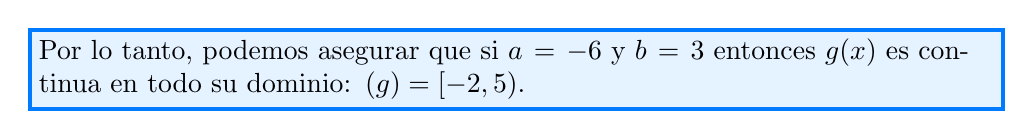
\begin{tikzpicture}
	\node[draw=lightblue, fill=lightblue!10, line width=1.5, text width=\linewidth] {Por lo tanto, podemos asegurar que si $a=-6$ y $b=3$ entonces $g(x)$ es continua en todo su dominio: $\dom(g)=[-2,5)$.};
\end{tikzpicture}
\end{enumerate}
\item \lb{Calcular el siguiente límite: \[ \lim_{x\to0}\dfrac{\sqrt{1+x}-\sqrt{1-x}}{x} \]}
$\lim_{x\to0}\dfrac{\sqrt{1+x}-\sqrt{1-x}}{x}=\left(\dfrac{0}{0}\right)=\left\{\begin{array}{l}
	\text{multiplicaremos y dividiremos}\\
	\text{por el conjugado de las raíces}
\end{array}\right\}=\lim_{x\to0}\dfrac{(\sqrt{1+x}-\sqrt{1-x})\cdot(\sqrt{1+x}-\sqrt{1-x})}{x(\sqrt{1+x}+\sqrt{1-x})}\linebreak=\lim_{x\to0}\dfrac{(\sqrt{1+x})^2-(\sqrt{1-x})^2}{x(\sqrt{1+x}+\sqrt{1-x})}=\lim_{x\to0}\dfrac{(\cancel{1}-x)-(\cancel{1}-x)}{x(\sqrt{1+x}+\sqrt{1-x})}=\lim_{x\to0}\dfrac{2\cancel{x}}{\cancel{x}(\sqrt{1+x}+\sqrt{1-x})}=\dfrac{2}{2}=\bboxed{1}$
\item \lb{Calcular el siguiente límite: \[ \lim_{x\to+\infty}\dfrac{3x^2+2}{x^2+3x+5} \]}

\begin{minipage}{0.5\textwidth}
	$\lim_{x\to+\infty}\dfrac{3x^2+2}{x^2+4x+5}=\left(\dfrac{\infty}{\infty}\right)=\lim_{x\to+\infty}\dfrac{\frac{3x^2}{x^2}+\frac{2}{x^2}}{\frac{x^2}{x^2}+\frac{3x}{x^2}+\frac{5}{x^2}}=\lim_{x\to+\infty}\dfrac{3+\tozero{\frac{2}{x^2}}}{1+\tozero{\frac{3}{x}}+\tozero{\frac{5}{x^2}}}=\bboxed{3}$
\end{minipage}\qquad\begin{minipage}{0.4\textwidth}
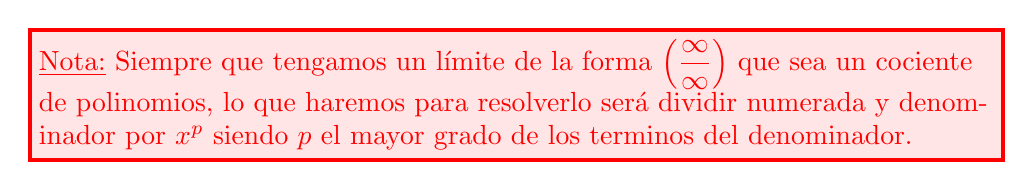
\begin{tikzpicture}
	\node[red, draw=red, fill=red!10, line width=1.5, text width=\linewidth] {\underline{Nota:} Siempre que tengamos un límite de la forma $\left(\dfrac{\infty}{\infty}\right)$ que sea un cociente de polinomios, lo que haremos para resolverlo será dividir numerada y denominador por $x^p$ siendo $p$ el mayor grado de los terminos del denominador.};
\end{tikzpicture}
\end{minipage}
\item \lb{Calcular el siguiente límite: \[ \lim_{x\to+\infty}\dfrac{3x}{x^2+2} \]}
$\lim_{x\to+\infty}\dfrac{3x}{x^2+2}=\left(\dfrac{\infty}{\infty}\right)=\lim_{x\to+\infty}\dfrac{\frac{3x}{x^2}}{\frac{x^2}{x^2}+\frac{2}{x^2}}=\lim_{x\to+\infty}\dfrac{\tozero{\frac{3}{x}}}{1+\tozero{\frac{2}{x^2}}}=\dfrac{0}{1}=\bboxed{0}$
\item \lb{Calcular el siguiente límite: \[ \lim_{x\to+\infty}\left(\dfrac{x+1}{x-1}\right)^x \]}
\begin{minipage}{0.55\textwidth}
	$\lim_{x\to+\infty}\left(\dfrac{x+1}{x-1}\right)^x=(1^\infty)=e^{\displaystyle\lim_{x\to0}x\left[\frac{x+1}{x-1}-1\right]}=\lb{(\ast)}=\bboxed{e^2}$
	
	\lb{\underline{Base:}\\
	$\lim_{x\to+\infty}\dfrac{x+1}{x-1}=\lim_{x\to+\infty}\dfrac{\frac{x}{x}+\tozero{\frac{1}{x}}}{\frac{x}{x}-\tozero{\frac{1}{x}}}=1$}
	
\end{minipage}\qquad\begin{minipage}{0.4\textwidth}
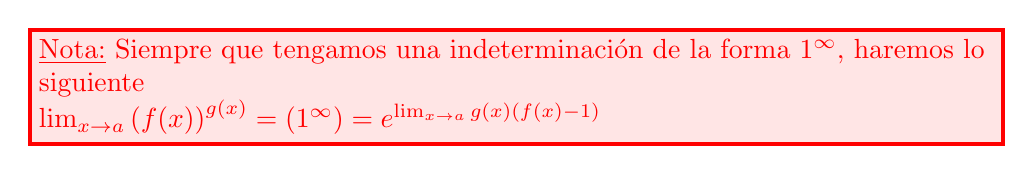
\begin{tikzpicture}
	\node[red, draw=red, fill=red!10, line width=1.5, text width=\linewidth] {\underline{Nota:} Siempre que tengamos una indeterminación de la forma $1^\infty$, haremos lo siguiente\\
	$\lim_{x\to a}\left(f(x)\right)^{g(x)}=(1^\infty)=e^{\lim_{x\to a}g(x)\left(f(x)-1\right)}$};
\end{tikzpicture}
\end{minipage}
	
	$\lb{(\ast)=} \lim_{x\to+\infty}x\left[\dfrac{\cancel{x}+1-\cancel{x}+1}{x-1}\right]=\lim_{x\to+\infty}\dfrac{2x}{x-1}=\left(\dfrac{\infty}{\infty}\right)\dfrac{\frac{2x}{x}}{\frac{x}{x}-\tozero{\frac{1}{x}}}=2$
	
\item \lb{Calcular el siguiente límite: \[ \lim_{x\to+\infty}(\sqrt{x^2+1}-\sqrt{x^2-4}) \]}

$\lim_{x\to+\infty}(\sqrt{x^2+1}-\sqrt{x^2-4})=(\infty-\infty)=\lim_{x\to+\infty} \dfrac{(\sqrt{ x^{2}+1 })-(\sqrt{ x^{2}-4 })\cdot(\sqrt{ x^{2}+1 })+(\sqrt{ x^{2}-4 })}{(\sqrt{ x^{2}+1 })+(\sqrt{ x^{2}-4 })}=\linebreak\lim_{ x \to +\infty }\dfrac{(\sqrt{ x^{2}+1 })^{2}-(\sqrt{ x^{2}-4 })^2}{\sqrt{ x^{2}+1 }+\sqrt{ x^{2}-4 }}=\lim_{ x \to +\infty }\dfrac{(\cancel{x^{2}}+1)-(\cancel{x^{2}}-4)}{\sqrt{ x^{2}+1 }+\sqrt{ x^{2}-4  }}=\lim_{ x \to +\infty }\frac{5}{\sqrt{ x^{2}+1 }+\sqrt{ x^{2}-4 }}=\lim_{ x \to +\infty }\dfrac{5}{+\infty}=\bboxed{0}$
\item \lb{Estudiar la continuidad de la siguiente función: \[ f(x)=\begin{cases}
		\dfrac{1}{e^{\frac{1}{x-1}}+1} & \text{si }x\neq1\\
		1 & \text{si }x=1
	\end{cases} \]}

$\forall x\neq1\longrightarrow f(x)$ es continua por ser un cociente de funciones continuas con denominador distinto de cero.

Veamos si $f(x)$ es continua en $x=1$:
\end{enumerate}
\end{document}